%% Based on a TeXnicCenter-Template by Gyorgy SZEIDL.
%%%%%%%%%%%%%%%%%%%%%%%%%%%%%%%%%%%%%%%%%%%%%%%%%%%%%%%%%%%%%

%----------------------------------------------------------
%
%\documentclass{book}%
%
%----------------------------------------------------------
% This is a sample document for the standard LaTeX Book Class
% Class options
%       --  Body text point size:
%                        10pt (default), 11pt, 12pt
%       --  Paper size:  letterpaper (8.5x11 inch, default)
%                        a4paper, a5paper, b5paper,
%                        legalpaper, executivepaper
%       --  Orientation (portrait is the default):
%                        landscape
%       --  Printside:   oneside, twoside (default)
%       --  Quality:     final(default), draft
%       --  Title page:  titlepage, notitlepage
%       --  Columns:     onecolumn (default), twocolumn
%       --  Start chapter on left:
%                        openright(no, default), openany
%       --  Equation numbering (equation numbers on right is the default):
%                        leqno
%       --  Displayed equations (centered is the default):
%                        fleqn (flush left)
%       --  Open bibliography style (closed bibliography is the default):
%                        openbib
% For instance the command
          \documentclass[a4paper,12pt,reqno]{book}
% ensures that the paper size is a4, fonts are typeset at the size 12p
% and the equation numbers are on the right side.
%
\usepackage{amsmath}%
\usepackage{amsfonts}%
\usepackage{amssymb}%
\usepackage{graphicx}
%----------------------------------------------------------
\newtheorem{theorem}{Theorem}
\newtheorem{acknowledgement}[theorem]{Acknowledgement}
\newtheorem{algorithm}[theorem]{Algorithm}
\newtheorem{axiom}[theorem]{Axiom}
\newtheorem{case}[theorem]{Case}
\newtheorem{claim}[theorem]{Claim}
\newtheorem{conclusion}[theorem]{Conclusion}
\newtheorem{condition}[theorem]{Condition}
\newtheorem{conjecture}[theorem]{Conjecture}
\newtheorem{corollary}[theorem]{Corollary}
\newtheorem{criterion}[theorem]{Criterion}
\newtheorem{definition}[theorem]{Definition}
\newtheorem{example}[theorem]{Example}
\newtheorem{exercise}[theorem]{Exercise}
\newtheorem{lemma}[theorem]{Lemma}
\newtheorem{notation}[theorem]{Notation}
\newtheorem{problem}[theorem]{Problem}
\newtheorem{proposition}[theorem]{Proposition}
\newtheorem{remark}[theorem]{Remark}
\newtheorem{solution}[theorem]{Solution}
\newtheorem{summary}[theorem]{Summary}
\newenvironment{proof}[1][Proof]{\textbf{#1.} }{\ \rule{0.5em}{0.5em}}




\usepackage[ngerman,english]{babel}	
\usepackage{caption} %% for \captionof{}{}
%%%%%%%%%%%%%%%%%%%%%%%%%%%%%%%%%%%%%%%%%%%%%%%%%%%%%%%%%%%
%\usepackage{fancyhdr}
%\pagestyle{fancy}


% new koma package
\usepackage{scrpage2}
%%%%%%%%%%%%%%%%%%%%%%%%%%%%%%%%%%%%%%%%%%%%%%%%%%%%%%%%%%%%
% for koma headers
\pagestyle{scrheadings}
% define head and foot marks
\renewcommand{\chaptermark}[1]{\markboth{#1}{}}
\renewcommand{\sectionmark}[1]{\markright{-~#1}{}}
%\ihead{\leftmark}
\ihead{}					%left head
\chead{\leftmark} %right head
\ohead{} 					%right head
%\ohead{\pagemark}
\ifoot{}
\cfoot{}
\ofoot{}
\setheadsepline{.4pt}



%define paralle typeset
%%%%%%%%%%%%%%%%%%%%%%%%%%%%%%%%%%%%%%%%%%%%%%%%%%%%%%%%%%%%%%%%%%%%%%%%%%%
\usepackage{parallel} % 2003/04/13
\usepackage{pdfcolparcolumns} % 2008/08/11
\usepackage{blindtext}
\newcommand\LR[0]{}
\renewcommand\LR[2]{\begin{Parallel}[c]{0.475\textwidth}{0.475\textwidth}%
    \selectlanguage{ngerman}\ParallelLText{#1}%    
    \selectlanguage{english}\ParallelRText{#2}%    
    \ParallelPar%
    \end{Parallel}%
    }

%----------------------------------------------------------
\begin{document}

\frontmatter
\title{The Title of the Book}
\author{Author{s}}
\date{The Date}
\maketitle
\tableofcontents


%%%%%%%%%%%%%%%%%%%%%%%%%%%%%%%%%%%%%%%%%%%%%%%%%%%%%
\pagenumbering{arabic}

\ihead{}					%left head
\chead{\leftmark} %right head
\ohead{} 					%right head
%\ohead{\pagemark}
\ifoot{}
\cfoot{\pagemark}
\ofoot{}

%mainmatter

\chapter{Vorwort}
%Preface

%\LR{
		%\subsection{sub1 Parallel} 
%		\blindtext 
%		}{
		%\esubsection{sub2 Parallel}
%		 \blindtext
%}

\chapter{Personal}
\echapter{STAFF}
%STAFF
%Emeritus
%Emrtitus
\section*{Emrtitus}
 
 \begin{minipage}[t]{\textwidth}
	\begingroup
	\parfillskip=0pt
	
  	\begin{minipage}[t]{0.25\textwidth}	
   		%\blindtext	
   		\centering
		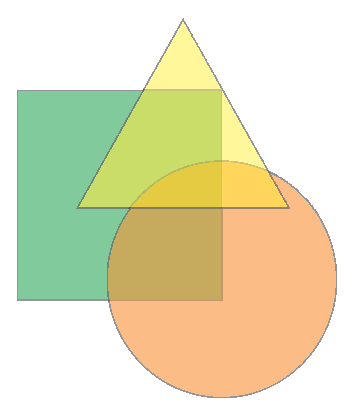
\includegraphics[width=0.7\textwidth]{Bilder/Grafik}		
		%\captionof{figure}{ Grafiken}	
			%\label{fig:GrafikOptionen}
  	\end{minipage}	
 	\hfill 	
  	\begin{minipage}[c]{0.7\textwidth}
  		\blindtext
  	\end{minipage}  
	\par\endgroup
\end{minipage}


% \begin{minipage}[t]{0.6\textwidth}
%	\begingroup
%	\parfillskip=0pt
%	% zwei weitere Minipages
%	\begin{minipage}[t]{0.47\textwidth}
%	\blindtext
%	\end{minipage}%
%	\hfill
%	\begin{minipage}[t]{0.47\textwidth}
%	\blindtext
%	\end{minipage}%
%	\par\endgroup
%\end{minipage}


%Technische Mitarbeiter und Sekretariat
%Technical staff and office
\newpage

\section*{Technische Mitarbeiter und Sekretariat}

	\begin{tabular}{p{2.1cm}p{6cm}p{2cm}p{6cm}}
	% 1. row
	\parbox[c]{2cm}{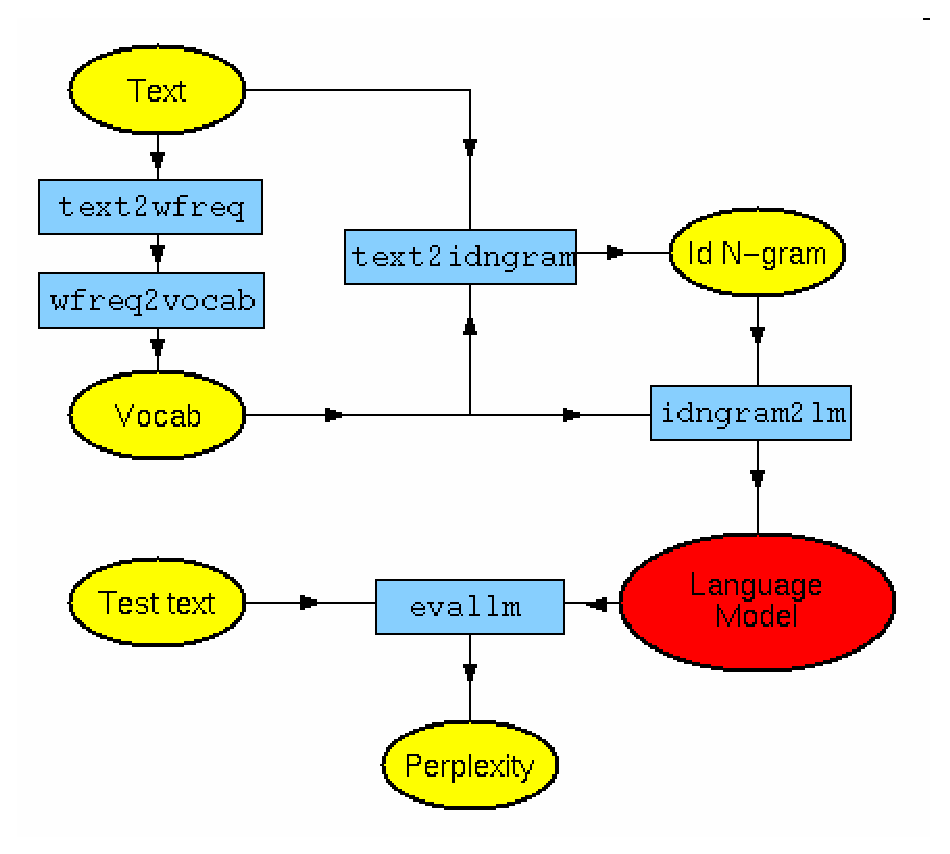
\includegraphics[width=2cm]{Bilder/toolkit.eps}} 	\hfill 	 	
	& \parbox[c]{5.9cm}{
			Dipl.Ing Wilhelm Peters\\
			Studium der Elektrotechnik\\
			\enfont{Studies in electrical engineering}\\
			Systemoptimierung Fahrantrieb\\
			\enfont{System optimisation traction drive}\\
			\phantom{test}\\
			\phantom{test}\\
		}	
	&	\parbox[c]{2cm}{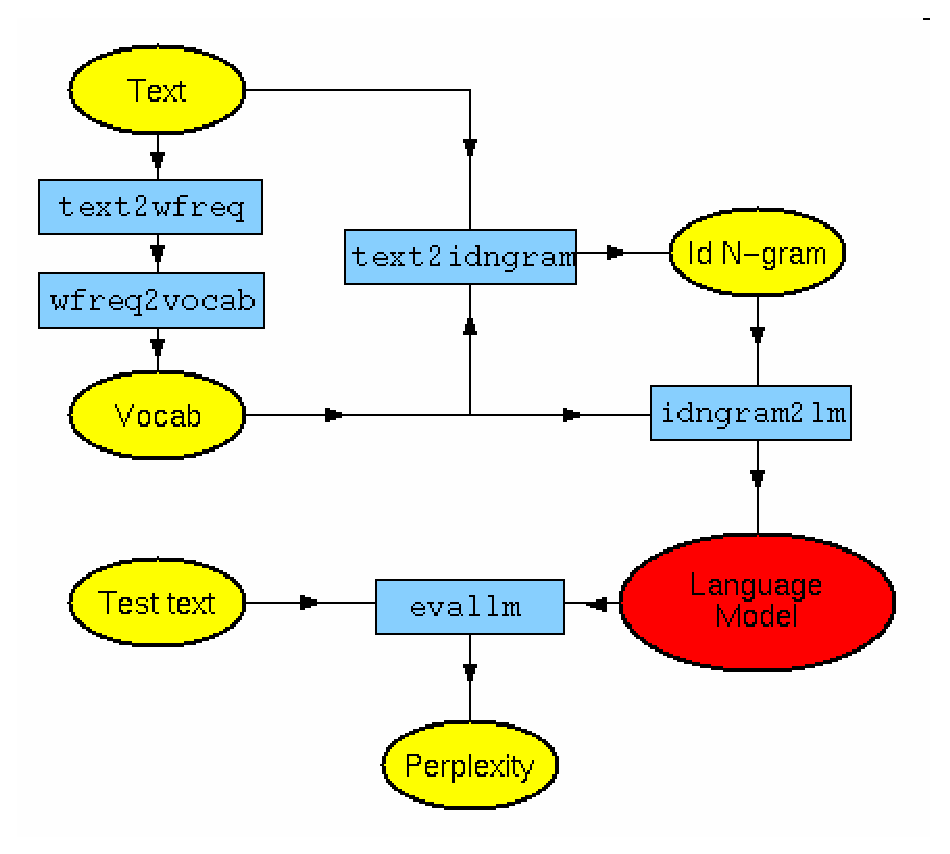
\includegraphics[width=2cm]{Bilder/toolkit.eps}}  	\hfill 		
	
	& \parbox[c]{5.9cm}{
			Dipl.Ing Wilhelm Peters\\
			Studium der Elektrotechnik\\
			\enfont{Studies in electrical engineering}\\
			Systemoptimierung Fahrantrieb\\
			\enfont{System optimisation traction drive}\\
			Mitarbeiter seit 2007
			\enfont{Member of staff since 2007}\\
		}\\
		%\phantom{Leerzeile} &&&\\
		
	% 2. row
	\parbox[c]{2cm}{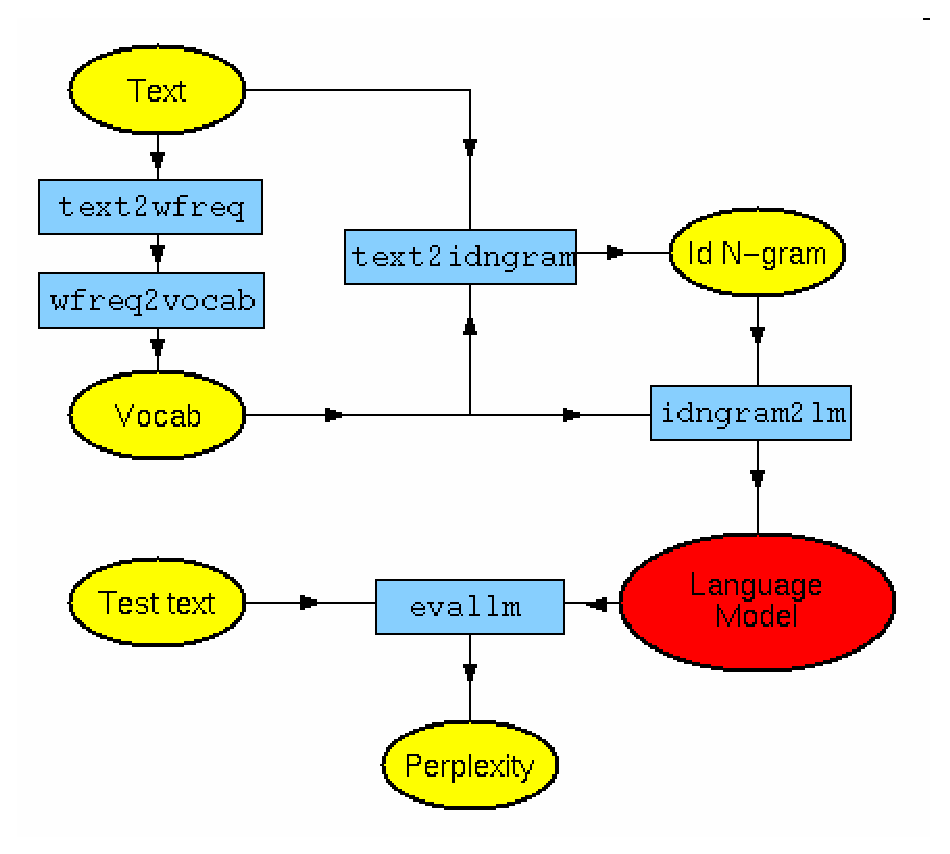
\includegraphics[width=2cm]{Bilder/toolkit.eps}} 	\hfill 	
	& \parbox[c]{5.9cm}{
			Dipl.Ing Wilhelm Peters\\
			Studium der Elektrotechnik\\
			\enfont{Studies in electrical engineering}\\
			Systemoptimierung Fahrantrieb\\
			\enfont{System optimisation traction drive}\\
			\phantom{test}\\
			\phantom{test}\\
		}	
		
	&	\parbox[c]{2cm}{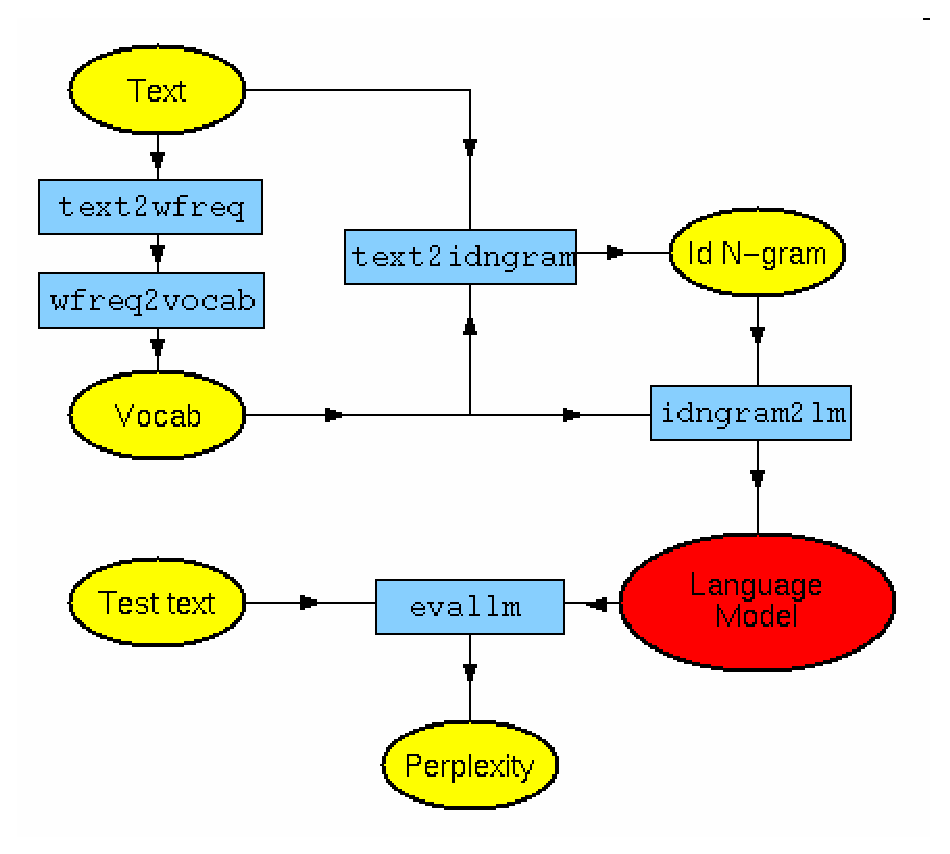
\includegraphics[width=2cm]{Bilder/toolkit.eps}}  	\hfill 	
	& \parbox[c]{5.9cm}{
			Dipl.Ing Wilhelm Peters\\
			Studium der Elektrotechnik\\
			\enfont{Studies in electrical engineering}\\
			Systemoptimierung Fahrantrieb\\
			\enfont{System optimisation traction drive}\\
			Mitarbeiter seit 2007
			\enfont{Member of staff since 2007}\\
		}\\
	%	\phantom{Leerzeile} &&&\\		
\end{tabular}
%Wissenschaftliche Mitarbeiter
%Scientific staff

\section*{Wissenschaftliche Mitarbeiter}

	\begin{tabular}{p{2.1cm}p{6cm}p{2cm}p{6cm}}
	% 1. row
	\parbox[c]{2cm}{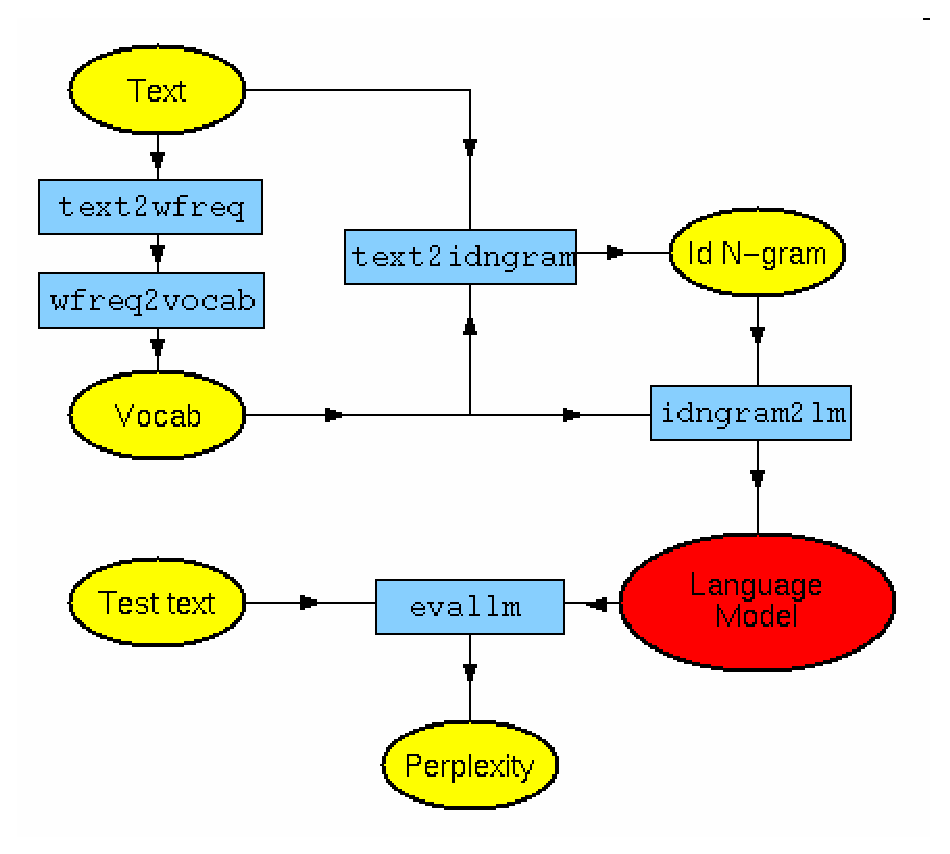
\includegraphics[width=2cm]{Bilder/toolkit.eps}} 	\hfill 	 	
	& \parbox[c]{5.9cm}{
			\Large Dipl.Ing Wilhelm Peters \normalsize \\
			\phantom{test}\\
			Studium der Elektrotechnik\\
			\enfont{Studies in electrical engineering}\\
			Systemoptimierung Fahrantrieb\\
			\enfont{System optimisation traction drive}\\
			\phantom{test}\\
			\phantom{test}\\
		}	
	&	\parbox[c]{2cm}{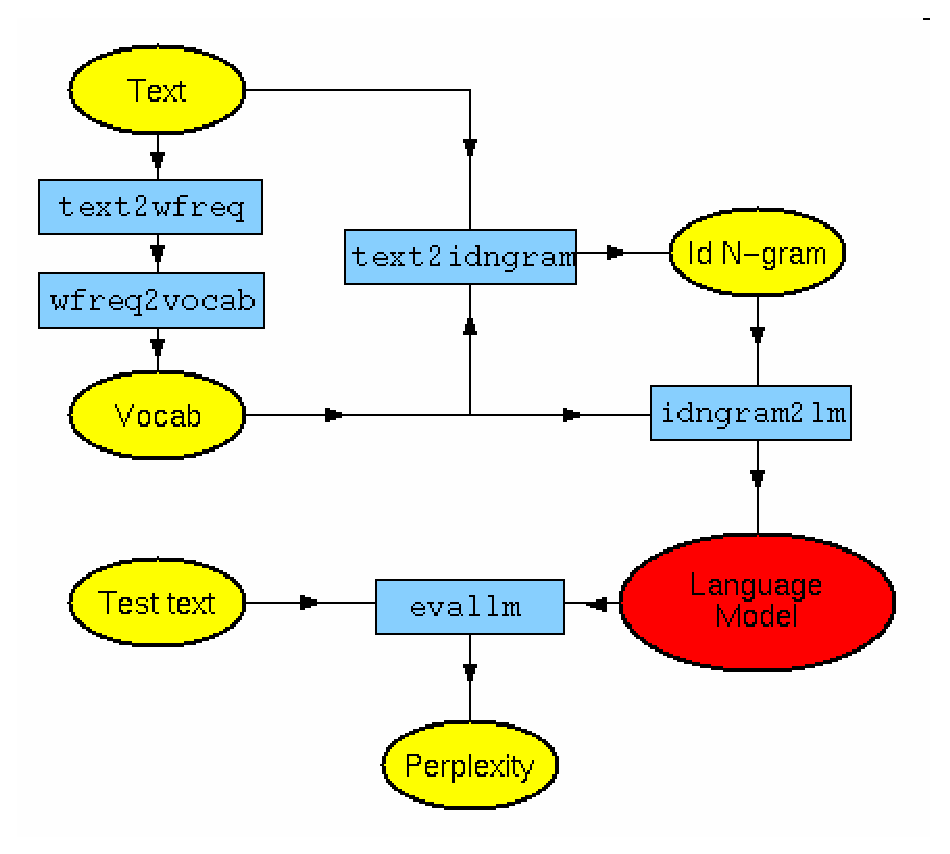
\includegraphics[width=2cm]{Bilder/toolkit.eps}}  	\hfill 		
	
	& \parbox[c]{5.9cm}{
			\Large Dipl.Ing Wilhelm Peters \normalsize \\
			\phantom{test}\\
			Studium der Elektrotechnik\\
			\enfont{Studies in electrical engineering}\\
			Systemoptimierung Fahrantrieb\\
			\enfont{System optimisation traction drive}\\
			Mitarbeiter seit 2007
			\enfont{Member of staff since 2007}\\
		}\\
		%\phantom{Leerzeile} &&&\\
		
	% 2. row
	\parbox[c]{2cm}{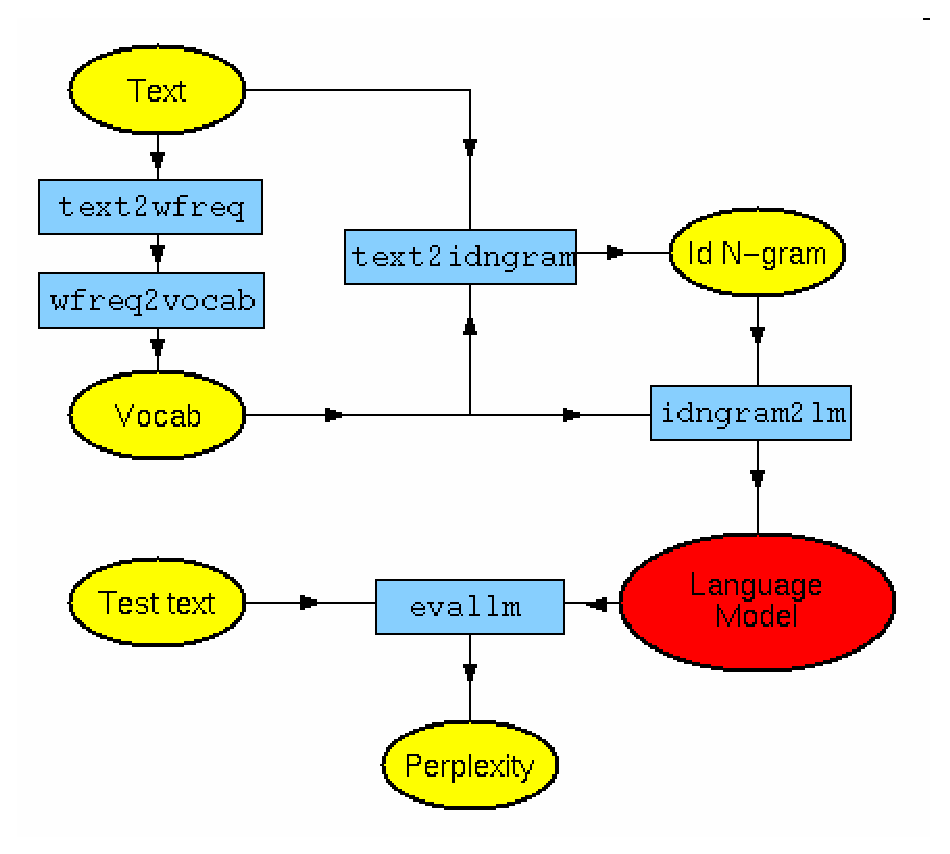
\includegraphics[width=2cm]{Bilder/toolkit.eps}} 	\hfill 	
	& \parbox[c]{5.9cm}{
			\Large Dipl.Ing Wilhelm Peters \normalsize \\
			\phantom{test}\\
			Studium der Elektrotechnik\\
			\enfont{Studies in electrical engineering}\\
			Systemoptimierung Fahrantrieb\\
			\enfont{System optimisation traction drive}\\
			\phantom{test}\\
			\phantom{test}\\
		}	
		
	&	\parbox[c]{2cm}{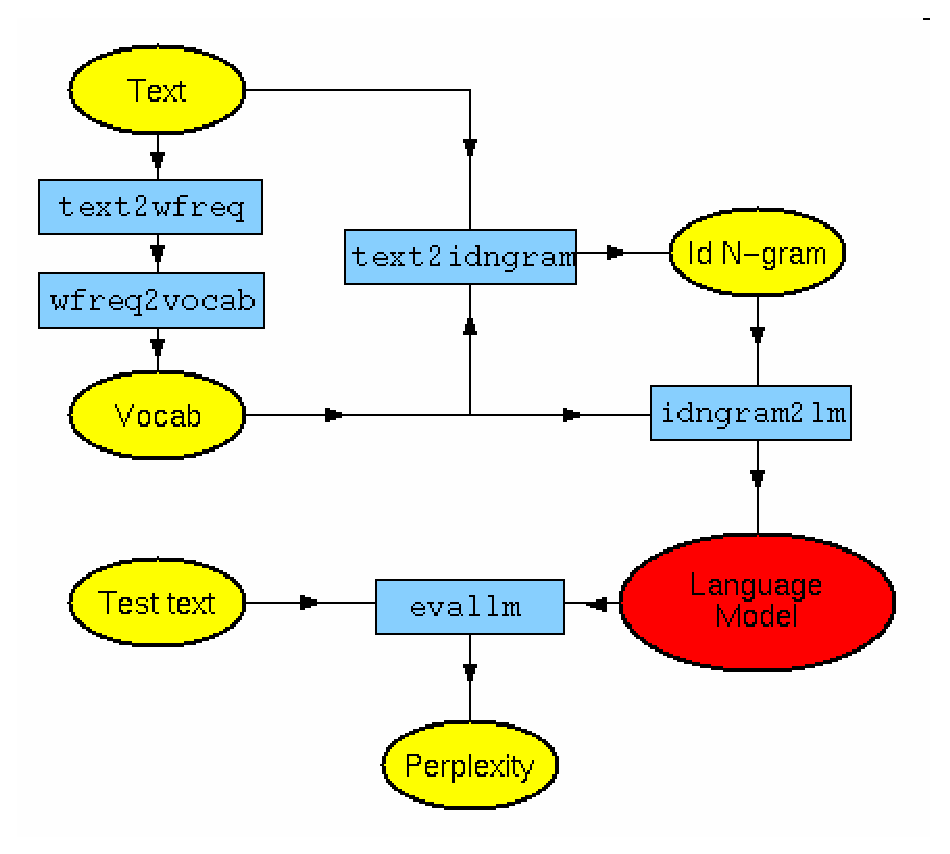
\includegraphics[width=2cm]{Bilder/toolkit.eps}}  	\hfill 	
	& \parbox[c]{5.9cm}{
			\Large Dipl.Ing Wilhelm Peters \normalsize \\
			\phantom{test}\\
			Studium der Elektrotechnik\\
			\enfont{Studies in electrical engineering}\\
			Systemoptimierung Fahrantrieb\\
			\enfont{System optimisation traction drive}\\
			Mitarbeiter seit 2007
			\enfont{Member of staff since 2007}\\
		}\\
	%	\phantom{Leerzeile} &&&\\		
\end{tabular}

Hier ist ein text. \phantom{Und hier ist der Text als phantom}. Hier ist wieder text.


\chapter{Forschungsschwepunkte}
\echapter{RESEARCH}
%\LR{
		%\subsection{sub1 Parallel} 
		%\blindtext \blindtext \blindtext \blindtext
%		}{
		%\esubsection{sub2 Parallel}
		% \blindtext \blindtext \blindtext \blindtext
%}
\input{mainmatter/forschungsschwepunkte/regelung_von_PM}

\chapter{Labor}
\echapter{Labory}


\chapter{Lehrveranstaltungen}



\chapter{Kooperationen}

%\clearpage
%\bibliographystyle{get_deu_alphadin}							% default styles  get_alphadin} %     
%\bibliographystyle{alpha}
%\bibliographystyle{get_natdin}
%\bibliographystyle{get_eng_natdin}						% f? englische Texte
%\bibliographystyle{unsrtdin}
%\bibliographystyle{bib/IEEEtran}
%\bibliography{bib/Ref_xby}

\begin{figure}
  \figbicaption{fig:test}{Deutscher Titel}{English Title}
\end{figure}



\chapter{Title of first chapter}
\begin{refsection}
This is just filler text \parencite{massa}.
This is just filler text \parencite{augustine}.
This is just filler text \parencite{cotton}.
This is just filler text \parencite{hammond}.
\printbibliography[heading=subbibliography]
\end{refsection}

\chapter{Title of second chapter}
\begin{refsection}
This is just filler text \parencite{hammond}.
This is just filler text \parencite{massa}.
This is just filler text \parencite{cotton}.
This is just filler text \parencite{murray}.
\printbibliography[heading=subbibliography]
\end{refsection}

\chapter{Title of third chapter}
\begin{refsection}
This is just filler text \parencite{murray}.
This is just filler text \parencite{augustine}.
This is just filler text \parencite{cotton}.
This is just filler text \parencite{bertram}.
\printbibliography[heading=subbibliography]
\end{refsection}

%%sample

\chapter*{Preface}

This is the preface and it is created using a TeX field in a
paragraph by itself containing \verb|\chapter*{Preface}|. When the
document is loaded, this appears if it were a normal chapter, but
it is actually an unnumbered chapter. The \verb|markboth| TeX
field at the beginning of this paragraph sets the correct page
heading for the Preface portion of the document. The preface does
not appear in the table of contents.

\chapter{Introduction}

The introduction is entered using the usual chapter command. Since
the introduction chapter appears before the \verb|mainmatter| TeX
field, it is again an unnumbered chapter. The primary difference
between the preface and the introduction in this sample document
is that the introduction will appear in the table of contents and
the page headings for the introduction are automatically handled
without the need for the \verb|markboth| TeX field. You may use
either or both methods to create chapters at the beginning of your
document. You may also delete these preliminary chapters.

\mainmatter

\part{The First Part}

\chapter{About the Standard Latex Book Class}

This is the body (mainmatter) of the Standard LaTeX Book document.

The front matter has a number of sample entries that you should
replace with your own.

Replace this text with the body of your book. Do not delete the
\verb|mainmatter| TeX field found above in a paragraph by itself
or the numbering of different objects will be wrong.

The typesetting specification selected by this document uses the
default class options. There are, however, a number of class
options. The available options include setting the paper size and
the point size of the font used in the body of the document etc.
Details are given as comments right after the \verb|documentclass|
command.

\chapter{The Most Important Features of this Document}

\section{Section}

Use the \verb"\section{Section}" command for major sections, and the
\verb"\subsection{Subsection}" command for subsections, etc.

\subsection{Subsection}

This is just some text under a subsection.

\subsubsection{Subsubsection}

This is just some text under a subsubsection.

\paragraph{Subsubsubsection}

This is just some  text under a subsubsubsection.

\subparagraph{Subsubsubsubsection}

This is just some text under a subsubsubsubsection.

\section{Typesetting Commands}

SSelect a part of the text then click on the button Emphasize (H!), or Bold (Fs), or
Italic (Kt), or Slanted (Kt) to typeset \emph{Emphasize}, \textbf{Bold},
\textit{Italics}, \textsl{Slanted} texts.

You can also typeset \textrm{Roman}, \textsf{Sans Serif}, \textsc{Small Caps}, and
\texttt{Typewriter} texts.

You can also apply the special, mathematics only commands $\mathbb{BLACKBOARD}$
$\mathbb{BOLD}$, $\mathcal{CALLIGRAPHIC}$, and $\mathfrak{fraktur}$. Note that
blackboard bold and calligraphic are correct only when applied to uppercase letters A
through Z.

You can apply the size tags -- Format menu, Font size submenu -- {\tiny tiny},
{\scriptsize scriptsize}, {\footnotesize footnotesize}, {\small small}, {\normalsize
normalsize}, {\large large}, {\Large Large}, {\LARGE LARGE}, {\huge huge} and {\Huge
Huge}.

You can use the \verb"\begin{quote} etc. \end{quote}" environment for typesetting
short quotations. Select the text then click on Insert, Quotations, Short Quotations:

\begin{quote}
The buck stops here. \emph{Harry Truman}

Ask not what your country can do for you; ask what you can do for your
country. \emph{John F Kennedy}

I am not a crook. \emph{Richard Nixon}

I did not have sexual relations with that woman, Miss Lewinsky. \emph{Bill Clinton}
\end{quote}

The Quotation environment is used for quotations of more than one paragraph. Following
is the beginning of \emph{The Jungle Books} by Rudyard Kipling. (You should select
the text first then click on Insert, Quotations, Quotation):

\begin{quotation}
It was seven o'clock of a very warm evening in the Seeonee Hills when Father Wolf woke
up from his day's rest, scratched himself, yawned  and spread out his paws one after
the other to get rid of sleepy feeling in their tips. Mother Wolf lay with her big gray
nose dropped across her four tumbling, squealing cubs, and the moon shone into the
mouth of the cave where they all lived. ``\emph{Augrh}'' said Father Wolf, ``it is time
to hunt again.'' And he was going to spring down hill when a little shadow with a bushy
tail crossed the threshold and whined: ``Good luck go with you, O Chief of the Wolves;
and good luck and strong white teeth go with the noble children, that they may never
forget the hungry in this world.''

It was the jackal---Tabaqui the Dish-licker---and the wolves of India despise Tabaqui
because he runs about making mischief, and telling tales, and eating rags and pieces of
leather from the village rubbish-heaps. But they are afraid of him too, because
Tabaqui, more than any one else in the jungle, is apt to go mad, and then he forgets
that he was afraid of anyone, and runs through the forest biting everything in his way.
\end{quotation}

Use the Verbatim environment if you want \LaTeX\ to preserve spacing, perhaps when
including a fragment from a program such as:
\begin{verbatim}
#include <iostream>         // < > is used for standard libraries.
void main(void)             // ''main'' method always called first.
{
 cout << ''This is a message.'';
                            // Send to output stream.
}
\end{verbatim}
(After selecting the text click on Insert, Code Environments, Code.)


\section{Mathematics and Text}

It holds \cite{KarelRektorys} the following
\begin{theorem}
(The Currant minimax principle.) Let $T$ be completely continuous selfadjoint operator
in a Hilbert space $H$. Let $n$ be an arbitrary integer and let $u_1,\ldots,u_{n-1}$ be
an arbitrary system of $n-1$ linearly independent elements of $H$. Denote
\begin{equation}
\max_{\substack{v\in H, v\neq
0\\(v,u_1)=0,\ldots,(v,u_n)=0}}\frac{(Tv,v)}{(v,v)}=m(u_1,\ldots, u_{n-1})
\label{eqn10}
\end{equation}
Then the $n$-th eigenvalue of $T$ is equal to the minimum of these maxima, when
minimizing over all linearly independent systems $u_1,\ldots u_{n-1}$ in $H$,
\begin{equation}
\mu_n = \min_{\substack{u_1,\ldots, u_{n-1}\in H}} m(u_1,\ldots, u_{n-1}) \label{eqn20}
\end{equation}
\end{theorem}
The above equations are automatically numbered as equation (\ref{eqn10}) and
(\ref{eqn20}).


\section{Lists Environments}

You can create numbered, bulleted, and description lists
(Use the Itemization or Enumeration buttons, or click on the Insert menu
then chose an item from the Enumeration submenu):

\begin{enumerate}
\item List item 1

\item List item 2

\begin{enumerate}
\item A list item under a list item.

\item Just another list item under a list item.

\begin{enumerate}
\item Third level list item under a list item.

\begin{enumerate}
\item Fourth and final level of list items allowed.
\end{enumerate}
\end{enumerate}
\end{enumerate}
\end{enumerate}

\begin{itemize}
\item Bullet item 1

\item Bullet item 2

\begin{itemize}
\item Second level bullet item.

\begin{itemize}
\item Third level bullet item.

\begin{itemize}
\item Fourth (and final) level bullet item.
\end{itemize}
\end{itemize}
\end{itemize}
\end{itemize}

\begin{description}
\item[Description List] Each description list item has a term followed by the
description of that term.

\item[Bunyip] Mythical beast of Australian Aboriginal legends.
\end{description}

\section{Theorem-Like Environments}

The following theorem-like environments (in alphabetical order) are available
in this style.

\begin{acknowledgement}
This is an acknowledgement
\end{acknowledgement}

\begin{algorithm}
This is an algorithm
\end{algorithm}

\begin{axiom}
This is an axiom
\end{axiom}

\begin{case}
This is a case
\end{case}

\begin{claim}
This is a claim
\end{claim}

\begin{conclusion}
This is a conclusion
\end{conclusion}

\begin{condition}
This is a condition
\end{condition}

\begin{conjecture}
This is a conjecture
\end{conjecture}

\begin{corollary}
This is a corollary
\end{corollary}

\begin{criterion}
This is a criterion
\end{criterion}

\begin{definition}
This is a definition
\end{definition}

\begin{example}
This is an example
\end{example}

\begin{exercise}
This is an exercise
\end{exercise}

\begin{lemma}
This is a lemma
\end{lemma}

\begin{proof}
This is the proof of the lemma.
\end{proof}

\begin{notation}
This is notation
\end{notation}

\begin{problem}
This is a problem
\end{problem}

\begin{proposition}
This is a proposition
\end{proposition}

\begin{remark}
This is a remark
\end{remark}

\begin{summary}
This is a summary
\end{summary}

\begin{theorem}
This is a theorem
\end{theorem}

\begin{proof}
[Proof of the Main Theorem]This is the proof.
\end{proof}

\appendix

\chapter{The First Appendix}

The \verb"\appendix" command should be used only once. Subsequent appendices can
be created using the Chapter command.

\chapter{The Second Appendix}

Some text for the second Appendix.

This text is a sample for a short bibliography. You can cite a book by making use of
the command \verb"\cite{KarelRektorys}": \cite{KarelRektorys}. Papers can be cited
similarly: \cite{Bertoti97}. If you want multiple citations to appear in a single set
of square brackets you must type all of the citation keys inside a single citation,
separating each with a comma. Here is an example: \cite{Bertoti97, Szeidl2001,
Carlson67}.

\begin{thebibliography}{9}
\bibitem {KarelRektorys}Rektorys, K., \textit{Variational methods in Mathematics,
Science and Engineering}, D. Reidel Publishing Company,
Dordrecht-Hollanf/Boston-U.S.A., 2th edition, 1975

\bibitem {Bertoti97} \textsc{Bert\'{o}ti, E.}:\ \textit{On mixed variational formulation
of linear elasticity using nonsymmetric stresses and displacements}, International
Journal for Numerical Methods in Engineering., \textbf{42}, (1997), 561-578.

\bibitem {Szeidl2001} \textsc{Szeidl, G.}:\ \textit{Boundary integral equations for
plane problems in terms of stress functions of order one}, Journal of Computational and
Applied Mechanics, \textbf{2}(2), (2001), 237-261.

\bibitem {Carlson67}  \textsc{Carlson D. E.}:\ \textit{On G\"{u}nther's stress functions
for couple stresses}, Quart. Appl. Math., \textbf{25}, (1967), 139-146.
\end{thebibliography}

\backmatter

\chapter{Afterword}

The back matter often includes one or more of an index, an afterword,
acknowledgements, a bibliography, a colophon, or any other similar item. In
the back matter, chapters do not produce a chapter number, but they are
entered in the table of contents. If you are not using anything in the back
matter, you can delete the back matter TeX field and everything that follows it.

\end{document}
